\documentclass[UTF8]{ctexart}
\usepackage{bookmark}
\usepackage{geometry}
\usepackage{hyperref}
\geometry{a4paper,scale=0.8}
\usepackage{ctex}
\usepackage{booktabs}
\usepackage{array}
\usepackage{fancyhdr}
\pagestyle{fancy}
\fancyhf{}
\renewcommand\footrulewidth{1pt}
\lhead{\textit{王铠泽}}
\rhead{\textit{PB18020766}}
\chead{\href{mailto:volar@mail.ustc.edu.cn}{\textit{volar@mail.ustc.edu.cn}}}
\rfoot{\href{http://en.ustc.edu.cn/}{\textit{中国科学技术大学}}}
\lfoot{\today}
\usepackage{graphicx}
\usepackage{float}
\usepackage{subfigure}
\fancyfoot[C]{\thepage}


\begin{document}

	\centering\textbf{\LARGE{计算物理A第十二次作业}}
	
	\pagenumbering{arabic}
	\textit{王铠泽\qquad PB18020766}
	
		
	\section{作业题目}
	
	\begin{itemize}
	\item	推导三角格子点阵上座逾渗的重整化群变换表达式 $ p' = R(p) $,其中端-端连接
	的条件是3个格点中的2个是占据态,求临界点 $ p_c $ 与临界指数 $ \nu$,与正确值(表1.6.1.3-1)相比较。
	\end{itemize}

	\section{实现方法和原理}
	
	\begin{itemize}
		\item 重整化群方法
		
		重整化的基本思想就是对体系的长度尺
		度连续不断地做变换,将体系元胞尺度由$a$变换成$ ba $ ($ ba $ 应小于体系的相关长度$\xi$),相继标度变换的结果产生出一个流向图,空间流向场趋向于若干特殊的不动点,这些点在标度变换下保持不变。
		
		\item 三角格子的重整化
		
		对于二维的三角格子,$b=(N)^{1/d}=\sqrt{3}$。具体尺度变化如下图:
		
				\begin{figure}[H]
						\centering  %图片全局居中
						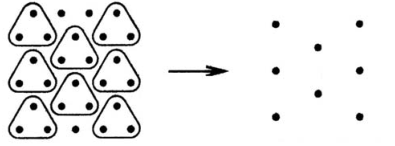
\includegraphics[width=4in]{../result/1.png}
						\caption{重整化尺度变换}
					\end{figure}
		根据题目描述,某个重整化后的个点导通对应的条件为至少两个原格点被占据,如下图的四种情况:
		
			\begin{figure}[H]
			\centering  %图片全局居中
			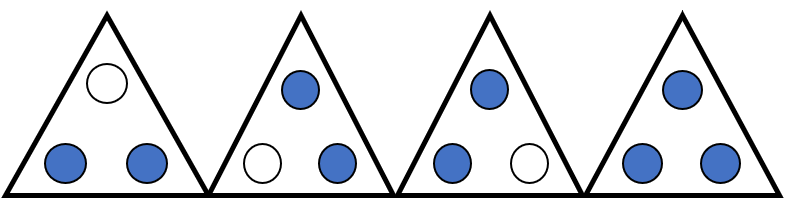
\includegraphics[width=4in]{../result/2.png}
			\caption{导通条件(蓝色填充表示被占据)}
		\end{figure}
	
	\item 临界点$p_c$计算
	
	由上面导通条件,可以得到重整化后每一个格点导通的概率为:
	
	$$p'=R(p)=p^3+3p^2(1-p)=-2p^3+3p^2$$
	
	临界点(不动点)$p_c$满足:
	
	$$p_c=-2p_c^3+3p_c^2$$
	
	求解这个方程,得到:
	
	$$p_c=0.5,p_0=0,p_1=1$$
	
	0和1是平凡解,我们所关注的是$p_c=0.5$,这才是临界点。
	
	\item 临界指数$\nu$计算
	
	重整化下的格子为了保持标度律不变,应当选择重整化后的关联长度$\xi'=\frac{\xi}{b}$。在接近$p_c$时,有$\xi(p)=|p-p_c|^{-\nu}$。所以:
	
	$$|p'-p_c|^{-\nu}=\frac{1}{b}|p-p_c|^{-\nu}$$
	
	而在$p_c$附近,有:
	
	$$p'-p_c=R(p)-R(p_c)=\lambda(p-p_c)$$
	其中$\lambda=\frac{dR(p)}{dp}|_{p=p_c}$
	
	$$\Rightarrow |p'-p_c|^{-\nu}=\lambda^{-\nu}|p-p_c|^{-\nu}$$
	
	$$\Rightarrow b=\lambda^{\nu}$$
	
	$$\Rightarrow \nu=\frac{ln(b)}{ln(\lambda)}$$
	
	带入上面计算的数据$p_c=0.5$,可以得到:
	
	$$\nu=\frac{ln\sqrt{3}}{ln(\frac{3}{2})}\approx1.354755646$$
	
	
	最后,将重整化计算得到的临界值和正确值进行比较:
	
	
	\begin{figure}[H]
		\centering  %图片全局居中
		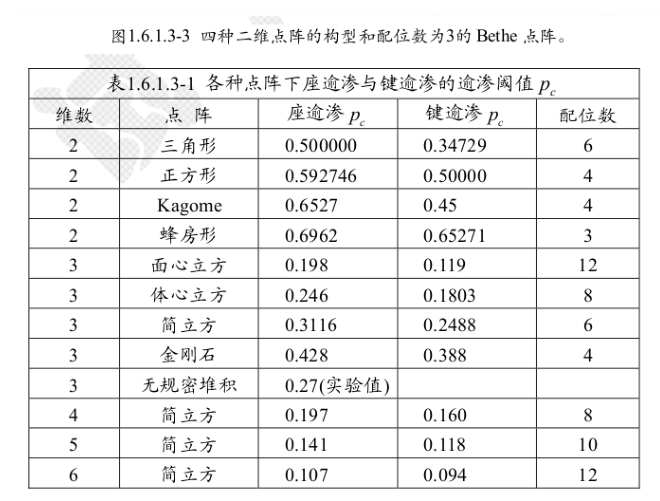
\includegraphics[width=6in]{../result/3.png}
		\caption{正确值表}
	\end{figure}

	可见$p_c$的座逾渗准确值为0.5,和我们用重整化的方法做出来的完全一致。
	
\end{itemize}

	

	\section{总结}
	\begin{itemize}
		\item 粗粒化近似,重整化群这一套方法是物理中重要的抓住本质的思想。对于相变理论,重整化往往能很好地计算出临界指数。本次作业就算一次很好的验证。
		\item 本次没有数值模拟环节,缺少对准确值的计算验证。等时间充裕,不失为一个很好的计算物理编程练习。
	\end{itemize}
	

\end{document}